\section{Lecture 28: The Hydrogen Atom}

Under classical mechanics, the hydrogen atom could not exist. If an electron has some velocity, it will
create a sinusoidal E-field and radiate light. The electron should then lose energy and spiral inwards to the center (in a very small amount of time!).

So Bohr posited that the radii of orbits are quantized. 
This means
\[ L_n = mvr_n = n\hbar \]

He also got from PLanck that energy is quantized units of $hf$, i.e. $f = \frac{E}{h}$.
Furthermore, any stable wave solution to an electron orbit must be a standing wave solution, i.e. that it is a periodic wave
which closes in on itself. $\lambda_{dB} = \frac{h}{p}$. Recall for a plane wave:
\[ e^{i(kx - \omega t)} \implies p = \hbar k = \frac{h}{\lambda}, E = \hbar \omega = hf \]
So we already see the connection. From the boundary condition:
\[ 2 \pi r = n \lambda = n(\frac{h}{mv}) \implies mvr = n\hbar \]
This gives us a justification that the radii of orbits are quantized. The centripetal force
is just a Coulomb force, with potential energy:
\begin{align*}
    U &= \frac{-e^2}{4\pi \epsilon r} \\
    &= \frac{-k_C e^2}{r}
\end{align*}
The total energy is:
\[ E = \frac{1}{2} mv^2 - \frac{k_Ce^2}{r^2} \]
and from Newton's second law:
\[ \frac{mv^2}{r^2} = \frac{k_Ce^2}{r^2} \implies v = \sqrt{\frac{k_Ce^2}{mr}} \]
This means the total energy is:
\[ E = \frac{-k_C e^2}{2r} \]
For the radii:
\[ r_n = \frac{n\hbar}{mv} = \frac{n\hbar}{m} \sqrt{\frac{mr_n}{k_Ce^2}} \implies r_n = \frac{n^2 \hbar^2}{mke^2}\]
For $n = 1$, the ground state orbit is called the Bohr radius $a_0$.
\[ r_1 = a_0 = \frac{\hbar^2}{m k_C e^2} \approx 0.529 \text{\r{A}} \]
The energies are:
\[ E_n = \frac{-k_C e^2}{2 a_0} \qty(\frac{1}{n^2}) = \frac{-13.6 \text{eV}}{n^2} \]
To rip off 1 electron, you need $13.6$ volts. These were both perfect for Hydrogen!
However, this is not robust to other systems and does not allow us to understand the time dynamics
of the system.

\subsection{The Wavefunction Viewpoint}
Let's try to solve it like one of our other problems. This is our setup:

Note that the potential is:
\[ V(r) = \frac{-ze^2}{4 \pi \epsilon_0 r} \]
which is central. We should also change into the center of mass frame.
Recall the reduced mass $\mu = \frac{mM}{m + M}$. From the point of view of the electron, all we care about is little $r$.

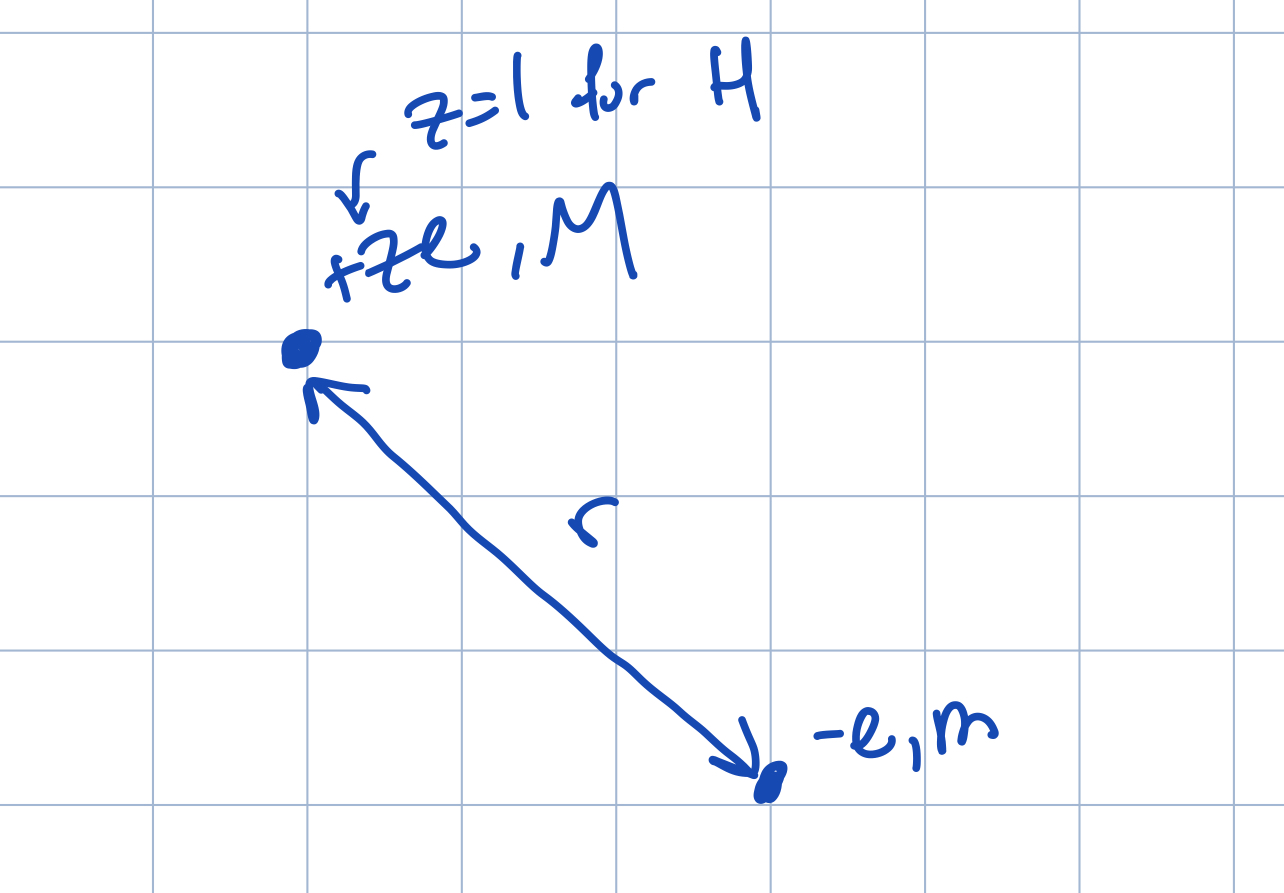
\includegraphics[width=200px]{twoparts.jpeg}

The Hamiltonian for the reduced coordinate $r$ is:
\[ \hat{H} = \frac{\hat{p}^2}{2\mu} - \frac{ze^2}{4\pi\epsilon_0 r} \]

This gives Schrodinger equation:
\begin{align*}
    [-\frac{\hbar^2}{2\mu}\nabla^2 - \frac{ze^2}{4\pi\epsilon_0 r}] \Psi(\mbf{r}) &= E \Psi(\mbf{r})
\end{align*}
We know for a central potential, this is separable:
\[ \Psi_{E\ell m}(\mbf{r}) = R_{E \ell}(r) Y_{\ell m}(\theta, \phi) \]
Where $Y$ is again the spherical harmonic. We write then write the Radial Equation with substitution $u_{E\ell}(r) = r R_{E\ell}(r)$
(TODO)
Where 
\[ V_{eff}(r) = V + \frac{\ell(\ell + 1)\hbar^2}{2\mu r^2} = \frac{-ze^2}{4\pi\epsilon_0 r} + \frac{\ell(\ell + 1)\hbar^2} 2\mu r^2\]
This creates a series of curves that looks like:

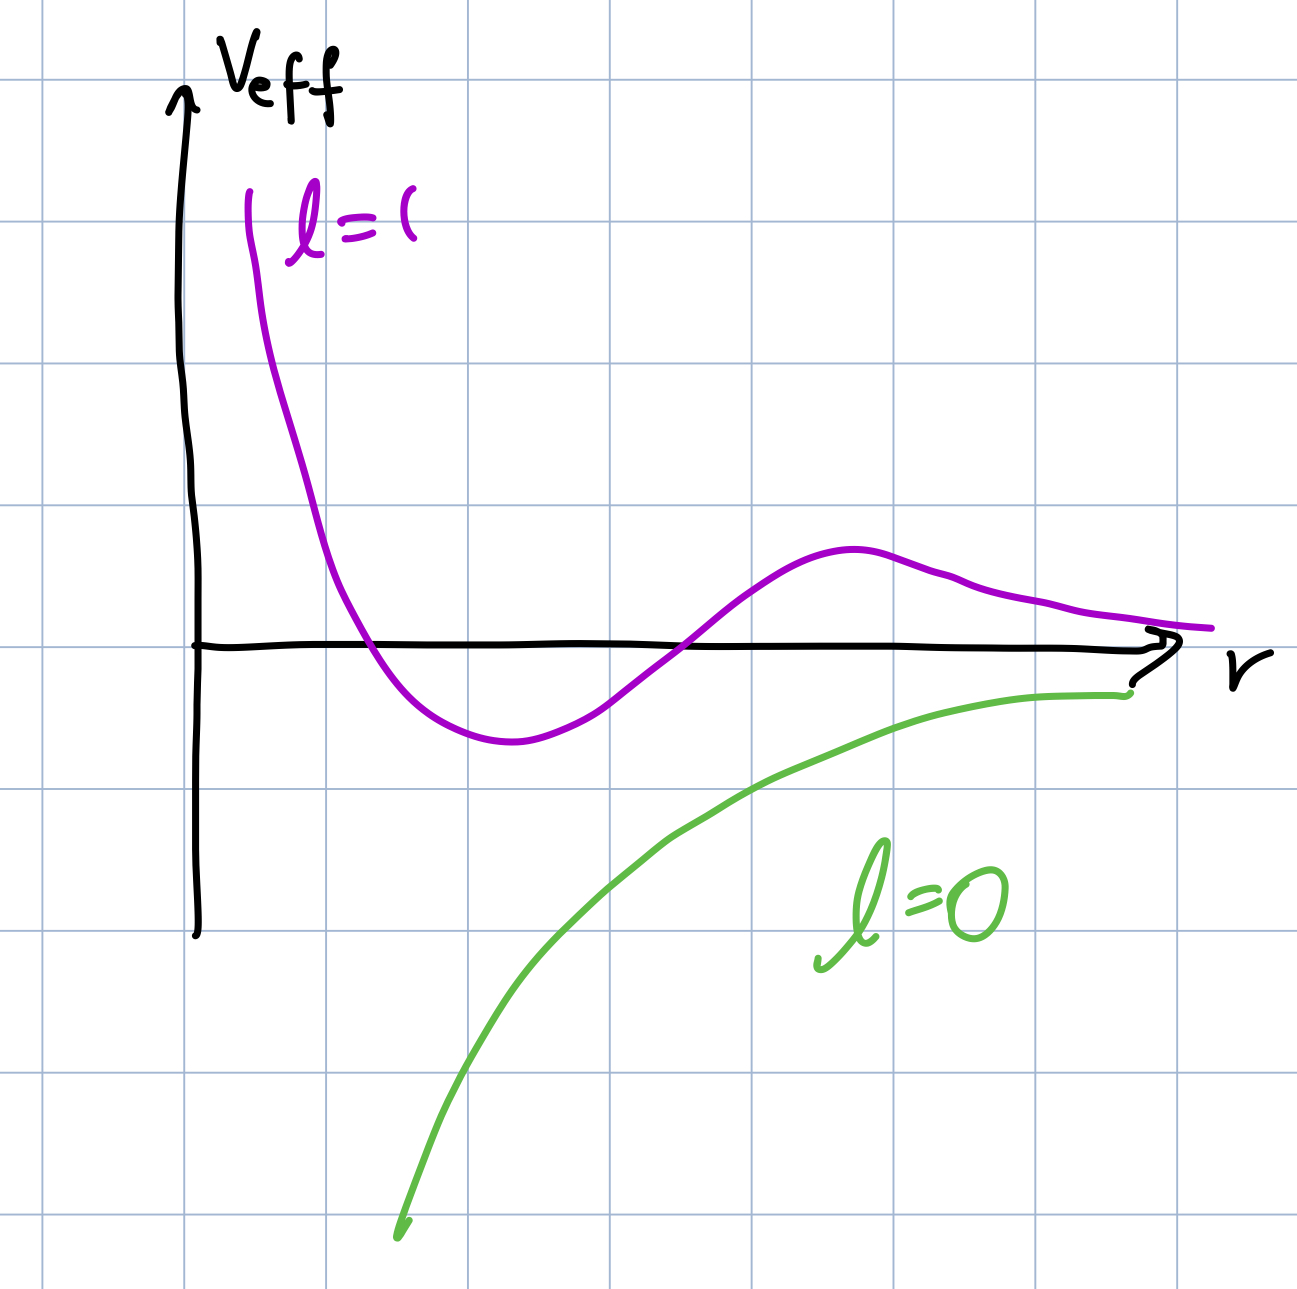
\includegraphics[width=300px]{effectivepot.jpeg}

For $E < 0$ we will get bound states, for $E > 0$ we will get scattering states.
The boundary condition must be that $u \to 0$ as $r \to \infty$ (since $R$ should )

Let
\begin{align*}
    \rho &= \qty(\frac{-8\mu E}{\hbar^2})^{1/2} r \\
    \lambda &= \frac{ze^2}{4\pi\epsilon_0 \hbar} \qty(\frac{-\mu}{2E})^{1/2} = z \alpha \qty(\frac{-\mu c^2}{2E})^{1/2} \\
    \qty[\dv{^2}{\rho^2} - \frac{\ell(\ell + 1)}{\rho^2} + \frac{\lambda}{\rho} - \frac{1}{4}] u(\rho) &= 0
\end{align*}

We will consider $\rho \to \infty$ and consider $\rho \to 0$ next lecture.

The steps we ended up following were:
\begin{enumerate}
    \item Draw a Picture
    \item Write Hamiltonian (use best coordinates)
    \item Write Schrodinger Equation
    \item Look for separable eigenstates $R_{E\ell}(r)$
    \item Write the Radial Equation with substitution $u_{E\ell}(r) = r R_{E\ell}(r)$
    \item Apply Boundary Conditions
    \item Simplify Equation with Redimensioning
    \item Solve the Equation
\end{enumerate}